Die Struktur der Software muss auf einen skill-basierten Ansatz ausgelegt werden. Dafür müssen die Anforderungen an eine solche Struktur klar definiert und die Möglichkeiten, die TwinCAT bietet, analysiert werden. In einem ersten Schritt wird die allgemeine Grobstruktur des Systems dargestellt (Abb. \ref{fig:Strukturübersicht}). Dieses kann wie folgt definiert werden: 

\begin{figure}[h!]
	\centering
	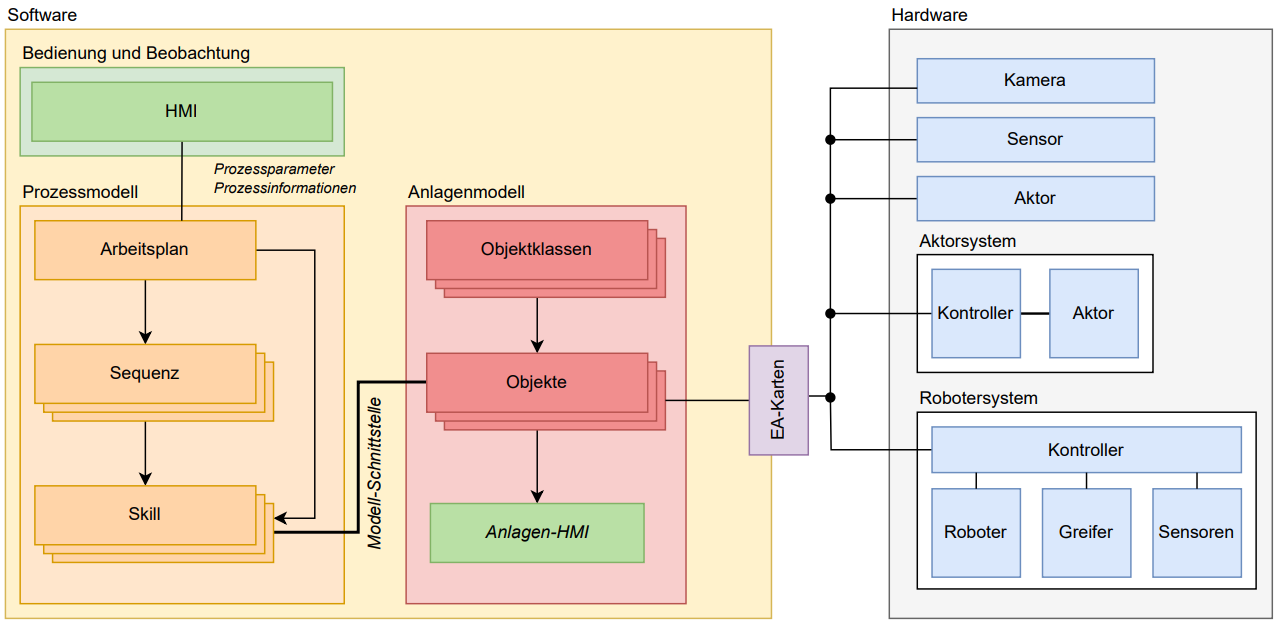
\includegraphics[width=1\textwidth]{05_Softwarestruktur/Overview}
	\captionsetup{justification=centering}
	\caption{Strukturübersicht}
	\label{fig:Strukturübersicht}
\end{figure}

Wie durch die ANSI/ISA-88-Norm vorgegeben (beschrieben in Kapitel \ref{Fragen bezüglich Referenzprojekt}), besteht die Software aus einem Prozess- und einem Anlagenmodell. Das Prozessmodell steuert den Ablauf, während das Anlagenmodell die Schnittstelle zu den einzelnen Anlagenkomponenten darstellt. Innerhalb des Prozessmodells werden die Skills definiert, die entweder von Sequenzen oder direkt aus dem Arbeitsplan zur Ablaufsteuerung genutzt werden können. Der Arbeitsplan beschreibt den gesamten Prozess.
\\
Das Anlagenmodell implementiert die Objektklassen der verschiedenen Systemelemente und bildet deren Funktionalitäten ab. Die Struktur des Anlagenmodells ist klar und übersichtlich: Die Objektklassen werden instanziiert und diese Objekte mit den entsprechenden Ein- und Ausgängen verknüpft, welche die Schnittstelle zum realen System darstellen. Der Grundgedanke dabei ist, dass alle Funktionalitäten zentral in der \Gls{SPS} gebündelt werden, um möglichst wenig Funktionalität auf den einzelnen Komponenten selbst zu belassen. Ziel ist es, dass sämtliche Elemente, von Robotern bis zu Kameras, über die \Gls{SPS} gesteuert werden können. Voraussetzung dafür ist, dass alle Komponenten über eine funktionale Schnittstelle zur \Gls{SPS} verfügen. Alle Komponenten werden im Anlagen-HMI visualisiert und können dort manuell gesteuert werden. Dies ermöglicht es beispielsweise, Roboterpositionen zu speichern, die später von einem Skill für Bewegungsabläufe genutzt werden können. 
\\
Abschliessend gibt es eine Bedienungs- und Beobachtungsebene, die als Benutzerschnittstelle dient, um Prozessparameter einzugeben und Informationen über den Prozess anzuzeigen. Diese Systemstruktur ermöglicht auch den modularen Aufbau von Systemen (Abb. \ref{fig:Gesamtsystemstruktur}). Das folgende Schema zeigt, wie ein solches System aussehen könnte:

\begin{figure}[h!]
	\centering
	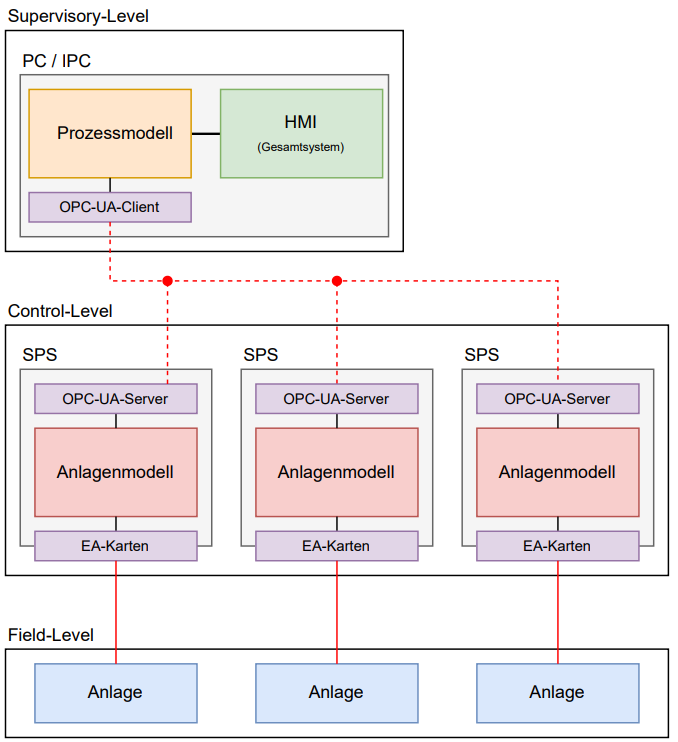
\includegraphics[width=0.5\textwidth]{05_Softwarestruktur/Gesamtsystemstruktur}
	\captionsetup{justification=centering}
	\caption{Gesamtsystemstruktur}
	\label{fig:Gesamtsystemstruktur}
\end{figure}

Das Schema orientiert sich an der Automatisierungspyramide \cite{Automatisierungspyramide} und zeigt die ersten drei Ebenen (Supervisory-, Control- und Field-Level). Dabei handelt es sich um ein System, welches aus verschiedenen Teilanlagen besten, mit eigener \Gls{SPS} und Anlagenmodell. Auf dem Supervisory-Level befindet sich das Prozessmodell. Hier wird über die HMI ein Arbeitsplan ausgewählt / zusammengestellt und gestartet. Eine OPC-UA-Schnittstelle übermittelt die prozessrelevanten Daten an die entsprechende \Gls{SPS} im Control-Level. Die \Gls{SPS} steuert die Anlage im Field-Level basierend auf dem Anlagenmodell. Die verschiedenen Anlagen können flexibel für unterschiedliche Aufgaben genutzt werden oder, falls sie identische Fähigkeiten besitzen, nach Auslastung zugewiesen werden. Dadurch ist das System äusserst flexibel und kann ohne grossen Aufwand erweitert werden.
